\section{Input data description}

 \subsection*{Map}
 Modeling means atomic interpretation of a map. This map can be the result of our own reconstruction process or can be obtained from a database. In this tutorial we use the haemoglobin map \ttt{EMD-3488}, that can be downloaded from \ttt{PDBE} (\url{http://www.ebi.ac.uk/pdbe/entry/emdb/EMD-3488}) (\ffigure{fig:PDBE}).\\
 WARNING in case you use your own map obtained from cryo-EM images: Take into account that cryo-EM 3D maps benefit significantly of an ``optimizing'' step, normally referred to as ``sharpening'' or ``density improvement``, that tends to increase signal at medium/high  resolution. Therefore, we recommend to sharp the map before tracing the atomic model. Either two \scipion protocols consecutively applied, \scommand{xmipp3 - local MonoRes} \citep{vilas2018} and \scommand{xmipp3 - localdeblur sharpening} \citep{ramirez2018}, or the protocol \scommand{xmipp3 - deepEMhancer} \citep{Sanchez-Garcia2020.06.12.148296}, allow map sharpening. Details about the parameters of these protocols are shown in Appendices \ref{app:localMonoRes}, \ref{app:localDeblurSharpening} and \ref{app:deepEMhancerSharpening}, respectively. 
 
 \begin{figure}[H]
  \centering
  \captionsetup{width=.8\linewidth} 
  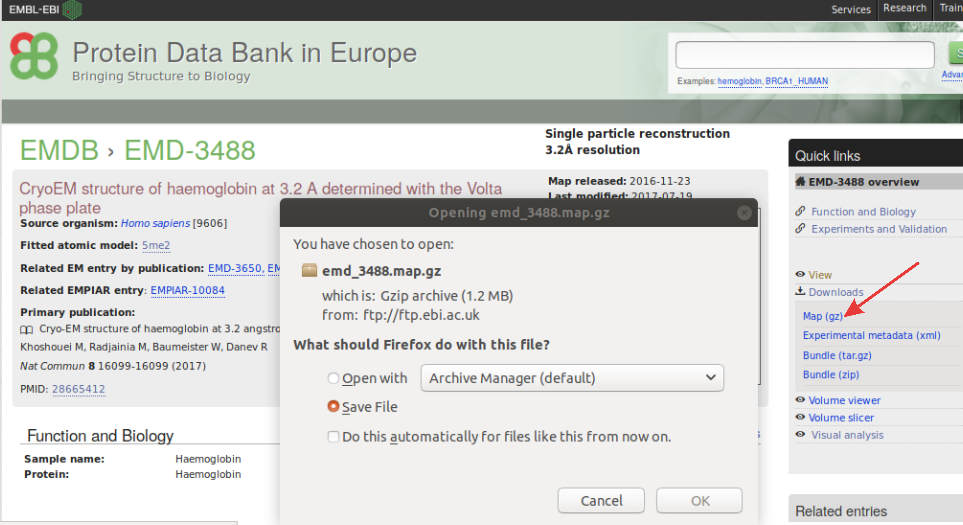
\includegraphics[width=0.95\textwidth]
  {{Images/Fig3}}
  \caption{Downloading the volume from \ttt{PDBe}.}
  \label{fig:PDBE}
  \end{figure}
  
  Once downloaded the volume, unpack it (command line: \ttt{gunzip emd-3488.map.gz}) and save it in your tutorial folder.
 
 \subsection*{Sequences}
 
 The sequences of \ttt{Hgb} $\alpha$ and $\beta$ subunits are included in \ttt{UniProtKB}. Accession numbers are \ttt{P69905} and \ttt{P68871}, respectively. Next, we show both sequences in fasta format:
 \begin{quote}
   \begin{verbatim}
>sp|P69905|HBA_HUMAN Haemoglobin subunit alpha
MVLSPADKTNVKAAWGKVGAHAGEYGAEALERMFLSFPTTKTYFPHFDLSHGSAQVKGHG
KKVADALTNAVAHVDDMPNALSALSDLHAHKLRVDPVNFKLLSHCLLVTLAAHLPAEFTP
AVHASLDKFLASVSTVLTSKYR

>sp|P68871|HBB_HUMAN Haemoglobin subunit beta
MVHLTPEEKSAVTALWGKVNVDEVGGEALGRLLVVYPWTQRFFESFGDLSTPDAVMGNPK
VKAHGKKVLGAFSDGLAHLDNLKGTFATLSELHCDKLHVDPENFRLLGNVLVCVLAHHFG
KEFTPPVQAAYQKVVAGVANALAHKYH
\end{verbatim}
 \end{quote}

 
 These protein sequences were determined by direct translation from the experimental sequence obtained from complementary \ttt{DNA (cDNA)}, i.e., \ttt{DNA} synthesized or retro-transcribed from messenger \ttt{RNA (mRNA)}. In this way, it is quite unlikely that these sequences include post-translational modifications. Although methionine is added with the translation \ttt{Met-tRNA} initiation factor, the removal of methionine aminoacid from the N-terminus of a polypeptide is a common post-translational modification. Since \ttt{Met} appears at the N-terminal end of both proteins, we can predict that these are not the polypeptide mature forms and \ttt{Met} will be removed in the mature ones that are present in the atomic structures. 
 
 Those two sequences can be retrieved from \ttt{UniProtKB} using \scipion\ \scommand{import sequence} protocol, which allows direct downloading from the database.
 

